\chapter{Databases and management}
In modern computing, \textbf{information} can be recorded in two ways:
\begin{itemize}
    \item as \textbf{structured data}, where the objects are represented by strings and numbers;
    \item as \textbf{unstructured data}, like in plain text.
\end{itemize}

When storing data, it's better to follow a structure. Every organization has its own way to manage information, from the storing to the processing and retrieval of data. We call the systems that manage data \textbf{Information Systems}.

\begin{definition}{Information System}
    An \textbf{Information System} is a \textbf{set of data} physically organized in secondary memory and managed in such a way as to allow its creation, updating and interrogation
\end{definition}

Back in the days, each organization would have its own file system, its own application written in different languages with different core ideas and different data management systems. The disadvantages are mostly the following three:
\begin{itemize}
    \item \textbf{redundancy}: while using the same data at the same time, two applications would create two copies of the same data;
    \item \textbf{inconsistency}: the update of an item would regard that only item, and not any other linked item;
    \item \textbf{data dependency}: its own organization would be on its own, since data would be stored in proprietary ways.
\end{itemize}

A solution was made with the creation of \textbf{databases}.

\begin{definition}{Database (DB)}
    A \textbf{database} is a set of mutually linked files. Data is organized in a data structure that facilitates the creation, the processing, the updating and the access of the resources. In order to handle a database, a \textbf{D}ata\textbf{b}ase \textbf{M}anagement \textbf{S}ystem (\textbf{DBMS}) is used
\end{definition}

Databases allow users to see in an abstract way the data that the users made. The goal of databases is to facilitate the processing of data, in relation to its properties. Generally, a database is an integrated resource shared by multiple components. It's important to establish integration and sharing between all users, but it's important to avoid concurrency (the simultaneous access to the same data)
\nwl
When talking about databases a lot of terms come to our mind: one of them is \textbf{queries}. Queries can be done in multiple ways and with multiple languages (for instance \textt{SQL}), but they all have a common basis: \textbf{relational algebra}. Queries are used to retrieve data from a database. All the properties shared between data are represented in a record structure.

\section{Data models}

Data is conceptually organized in \textbf{aggregates of homogeneous information} (so the \textbf{files}) that constitute the \textbf{components of the information system}, and each \textbf{update operation} is targeted to a \textbf{single aggregate} (to avoid redundancy), while a \textbf{query} may involve \textbf{one or more aggregates} (since it's a read-only process). Queries usually take advantages of \textbf{indexes}: they are files that allow to quickly retrieve information from a large quantity of files.
\nwl
There are various models that can be the basis of a database:
\begin{itemize}
    \item \textbf{logical models}: they are independent of the physical structures, but they are available in DBMS (some examples are networks, hierarchical models, relational models or object-oriented models);
    \item \textbf{conceptual models}: they are independent of the modalities of realization; their scope is to represent entities of the real world and their relations.
\end{itemize}

\subsection{Mesh model}

A common model is the \textbf{mesh model}, where data is usually represented as a collection of \textbf{records} of homogeneous type. Any \textbf{relationship} between data is represented as a \textbf{link} (more practically, links are made through pointers).
\nwl
A model is represented via a graph structure where:
\begin{itemize}
    \item the \textbf{nodes} are the \textbf{records};
    \item the \textbf{relationships} are the \textbf{links};
\end{itemize}

The most popular mesh system is \texttt{CODASYL}.

\subsection{Hierarchical model}

Another common model is the \textbf{hierarchical model}. Such model is a restricted type of mesh model, where each node has only one parent, and where a mesh is composed by a collection of trees (thus a forest). This last point guarantees hierarchy.

\subsection{Relational model}

In a relational model, each data and relationship is represented as values: there are no explicit references, so we will never see explicit pointers between data. Usually, relational models are used to have a high-level representation. In such models, objects are used to represent records, while all the field and attributes of such objects refer to any information of interest.

\subsection{Object model}

Such model is based on object and classes. Each attribute describes the state of an object, while methods describe the behaviour of an object. Each object encapsulates some attributes and behaviours. There is no universally recognised model yet.

\section{The three abstraction levels of a database}

Each database has three separate levels:
\begin{itemize}
    \item an \textbf{external schema}: it's the description of a portion of the database that allows different "views" of the database itself. The external schema depends on the access needs of each single user. The access to the database is granted only through the external schema, which may or may not coincide with the logical schema;
    \item a \textbf{logic schema}: it's the description of the entire database in the main logical models of the DBMS (for instance, the structure of the table);
    \item a \textbf{physical schema}: it's the representation of the logical schema by means of physical data structures.
\end{itemize}

\begin{center}
    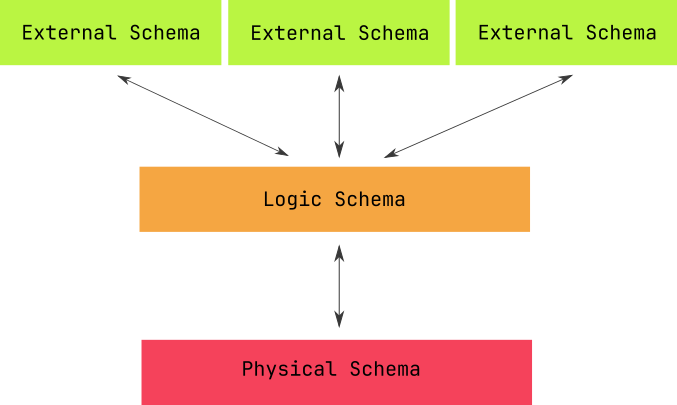
\includegraphics[scale = 0.45]{assets/images/DBLevels.png}
\end{center}

In a database there must be \textbf{physical} and \textbf{logical} independence:
\begin{itemize}
    \item \textbf{physical independence}: logical and external levels must be independent from the physical level. There must be the possibility to change the hardware without the need of changing also the software and the other two levels;
    \item \textbf{logical independence}: the external level is independent of the logical level, because the view of a user shouldn't affect the way data is organized. If one external level changes, it shouldn't change the logical organization.
\end{itemize}

Every database has its own \textbf{schema} (which must be \textbf{invariant} in time), which describes the database structure, and its own \textbf{instance}, which is an actual implementation of the schema. For instance, let the following table:

\begin{center}
    \begin{tabular}{|c|c|c|}
        \hline \rowcolor{maindoccol!60}
        \textbf{Name} & \textbf{Surname} & \textbf{Birth date} \\
        \hline
        Marco & Togni & 23/7/2003 \\
        \hline
        Alessandro & Borghese & 4/8/1998 \\
        \hline
        Joe & Biden & 6/11/1961 \\
        \hline
    \end{tabular}
\end{center}

We consider the first row as the scheme of our database, while the other rows with the data are the instances.
\nwl
While designing a database, it's important to keep \textbf{integrity}: there are, while designing a database, some constraints that have to be respected. For instance, a database used for university grades can't have negative values for the grades column, or in general it can't have any value outside the range $[18, 31]$.

\section{Database languages}

There are two types of languages that are used to interact with databases: 
\begin{itemize}
    \item \textbf{D}ata \textbf{D}efinition \textbf{L}anguage (\textbf{DDL}), which is used for the definition of schemes (be it a logical, an external or a physical scheme) and other general operations;
    \item \textbf{D}ata \textbf{M}anipulation \textbf{L}anguages (\textbf{DML}), which are used for querying and updating one or multiple instances of a database.
\end{itemize}

An example of language used with databases is the \textbf{S}tructured \textbf{Q}uery \textbf{L}anguage (\textbf{SQL}), which relies on the relational models. SQL integrates both DDL and DML in one unique language.

\section{Relational model in depth}

A relational model is based on the mathematical definition of relation. Each relation can be easily translated into tables. The relationships/associations between data are expressed as values. All values exist within a \textbf{domain}, which is a possibly infinite set of values (for instance the st of all integer numbers is a domain, but also $\{0, 1\}$ is a domain).

\begin{question}
    Now, let $D_1, D_2, \; ..., D_k$ be not necessarily distinct domains, then the Cartesian product, denoted by
    \[ D_1 \times D_2 \times ... \times D_k \]

    is the set
    \[ \left\{ (v_1, v_2, \;..., v_k) \; | \; v_1 \in D_1, v_2 \in D_2, \; ..., v_k \in D_k \right\} \]
\end{question}

A mathematical \textbf{relation} is any subset of the Cartesian product of one or more domains. A relation is said "of degree $k$" if such relation is a subset of a Cartesian product of $k$ domains. Each element of a relation is called \textbf{tuple} (or $n$-uples), and the \textbf{cardinality} of the relation is the number of tuples. Each tuple is distinct, and with the notation $t[i]$ we can select one component of the tuple among all the components. Indexes in this case start from 1.
\nwl
For instance, suppose that we have $k \eq 2$ domains. We could have for instance the following two domains:
\[ D_1 \eq \{ \text{white}, \text{ black} \} \quad \quad D_2 \eq \{ 0, 1, 2 \} \]

The Cartesian product of the two domain would be the following:
\[ D_1 \times D_2 \eq \{ (\text{white}, \; 0), \; (\text{white}, \; 1), \; (\text{white}, \; 2), \; (\text{black}, \; 0), \; (\text{black}, \; 1), \; (\text{black}, \; 2) \} \]

A possible relation could be for instance the following:
\[ r \eq \{ (\text{white}, \; 0), (\text{black}, \; 1), (\text{black}, \; 2) \} \]

Such relation has degree 2 and cardinality 3.
\nwl
It's really east to translate a relation into a table: for instance, let's translate the previous relation in a table:

\begin{center}
    $ r \eq \{ (\text{white}, \; 0), (\text{black}, \; 1), (\text{black}, \; 2) \}$ \hspace{20pt}
    \begin{tabular}{|c|c|}
        \hline
        white & 0 \\
        \hline
        black & 1 \\
        \hline
        black & 2 \\
        \hline
    \end{tabular}
\end{center}

We can interpret the data in the table by assigning names to the column and the table. The names are called \textbf{attributes}, which are defined by an \textbf{attribute name} $A$ and the related \textbf{domain} (denoted as $\text{dom}(A)$). An attribute simply assigns a readable name to a column, making it easier to understand what a column represents. The set of attributes creates a \textbf{relation schema}, which is usually indicated as follows:
\[ R(A_1, \; A_2, \; ..., \; A_k) \]

A set of relation schemas with different names is instead called \textbf{database schema}. From here, two other definitions can be made: first, the set of schemas $R_1, R_2, \;..., R_k$ is called \textbf{relational database schema}; second, the set of relation instances $\{r_1, r_2, \;..., r_k\}$ based on a schema $R_n$ is called \textbf{relational database}. Now, given these definitions, we can rearrange the previous table, making it become something like this:

\begin{center}
    Relations: 
    \begin{tabular}{|c|c|}
        \hline \rowcolor{maindoccol!60}
        \textbf{Colors} & \textbf{Numbers} \\
        \hline
        white & 0 \\
        \hline
        black & 1 \\
        \hline
        black & 2 \\
        \hline
    \end{tabular}
\end{center}

Mind that, once an order has been set, then it's not possible (or at least, not automatically) to change the order of the rows. If we change it, it doesn't really change regarding the content and the data, but mathematically, the order of the domains changed, thus it's a different table.

\begin{definition}{Ennuple on $R$}
    Let $R$ be a set of \textbf{attributes}: we call an \textbf{ennuple}, or tuple, \textbf{on} $R$ (denoted as $t$) a \textbf{function} that associates for each attribute $A \in R$ an element of $\text{dom}(A)$. The function $t(A)$ takes a value belonging to $\text{dom}(A)$ 
\end{definition}

In a relational model, the schema of a relation does not variate over time, since it describes its structure. Such aspect is called \textbf{intentional}.
\nwl
We call \textbf{instance} of a relation with a certain schema $R(X)$ a set $r$ of tuples on a set $X$ of attributes that contain some current values. More in general, it's an instance and practical application of the schema: it's a row of the database with its relative values. A \textbf{relation instance} is just the practical set of values that make a relation. Here follows an image with all the elements presented so far:

\begin{center}
    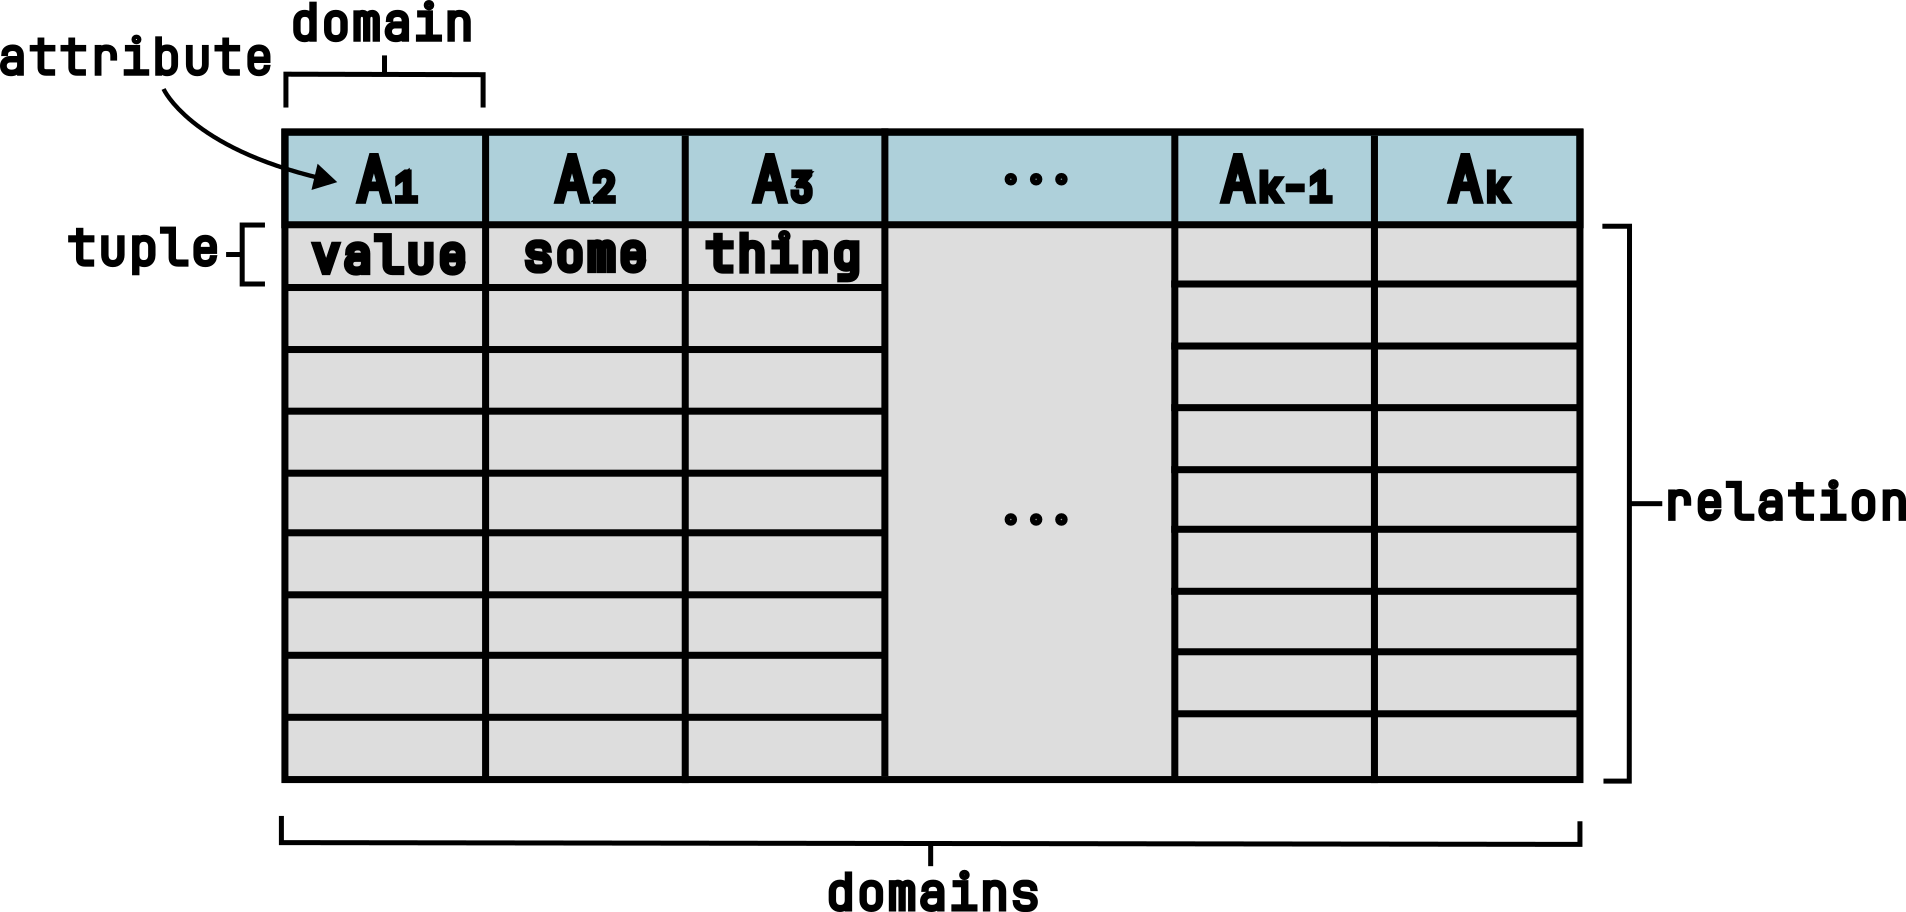
\includegraphics[scale = 0.30]{assets/images/DBElements.png}
\end{center}

In addition to all the elements presented before, we call a \textbf{database schema} a set of relation schemas which all have different names. Applied to the context of relational databases, a \textbf{relational database schema} is a set of relation schemas $R_1, \; R_2, \; ..., \; R_n$, while a \textbf{relational database} is the instance of a relational database schema, where $r_1, \; r_2, \; ..., \; r_n$ represent the relation instances or the corresponding relation schemas $R_1, \; R_2, \; ..., R_n$.

\begin{center}
    \begin{tabular}{|c|c|c|}
        \hline \rowcolor{maindoccol!60}
        \textbf{City} & \textbf{Region} & \textbf{Population} \\
        \hline
        Rome & Lazio, Italy & 3.000.000 \\
        \hline
        Milan & Lombardia, Italy & 2.000.000 \\
        \hline
        Brussel & Belgium & 1.220.000 \\
        \hline
        Antwerpen & Belgium & 506.000 \\
        \hline
    \end{tabular}
    \nwl
    An example of a relational database
\end{center}

If we want to define a precise item of a tuple, we can do it similarly on how dictionaries work in Python: given a tuple $t$, with $t[A_i]$ (where $A_i$ is the attribute relative to the element that we are defining), we denote the element. So in the previous case, if $t$ is the tuple of $\{ \text{"Brussel"}, \text{ "Belgium"}, \; 1.220.000 \}$, then with $t[\text{"Region"}]$ we are pointing to "Belgium". This operation has a precise name, and it's called \textbf{restriction}.

\begin{definition}{Restriction}
    Let $Y$ be a subset of attributes of a schema $X$, such that $Y \subseteq X$, then $t[Y]$ is the subset of values of the tuple $t$ that correspond to the attributes in $Y$. This operation is called \textbf{restriction}
\end{definition}

In a relational model, whenever there is a reference between two different relations, then such references are represented by means of  domain values that appear in the ennuples. So for instance, if we have the following three relational databases:

\begin{center}
    Students: \quad
    \begin{tabular}{|c|c|c|}
        \hline \rowcolor{maindoccol!60}
        \textbf{ID} & \textbf{Surname} & \textbf{Name} \\
        \hline
        0001 & Rossi & Mario \\
        \hline
        0002 & Monari & Lucia \\
        \hline
        0003 & Abili & Luca \\
        \hline
    \end{tabular}
    \hspace{25pt}
    Exams: \quad
    \begin{tabular}{|c|c|c|}
        \hline \rowcolor{maindoccol!60}
        \textbf{ID} & \textbf{Grade} & \textbf{Course} \\
        \hline
        0001 & 29 & CHEM1 \\
        \hline
        0002 & 26 & CALC1 \\
        \hline
        0003 & 30 & PROG1 \\
        \hline
    \end{tabular}
\end{center}

then the references between the two tables are given by $\text{dom}(\text{ID})$.

\subsection{The NULL value}

When a value is missing, we can't leave it blank, nor we can use 0 as filler. We need a specific value that is treated as a missing value. Such value is the \texttt{NULL} value. Called the "\textit{billion dollar mistake}" by Tony Hoare, its creator, the \texttt{NULL} value represents the \textbf{lack of information} or the \textbf{impossibility} to \textbf{apply a certain value to a certain domain}. In a database though, not all values should be able to be \texttt{NULL} (for instance the element ID). The \texttt{NULL} value doesn't belong to any specific domain, but it can replace any value in any domain (we call it \textbf{polymorphic value}).
\nwl
It's always important to use it whenever some data is missing or can't be made: unused values might be used later, and may have a meaning in a second time. The \texttt{NULL} value instead has a fixed meaning. Even in the same domain though, two \texttt{NULL} values have a different meaning.

\subsection{Constraints and keys}

When making a database, we must ensure some \textbf{integrity constraints}: they are properties that must be ensured by every instance of the database; they describe specific properties related to the scope of the constraint itself, thus to the information contained in the database. We say that a database instance is \textbf{correct} if it satisfies \textbf{all the integrity constraints} related to its schemas.
\nwl
If a constraint regards some elements in the same relation (thus either a single element of a tuple or some elements of the same tuple or relation), then such constraint is called \textbf{intra-relational constraint}, while if the constraint regards elements of two or more separate relations, then we call such constraint an \textbf{inter-relational constraint}.
\nwl
When dealing with relations, we may want to have a quick way that allows us to refer to each tuple. For instance, in a database with all the students in an university, there must be a way that allows us to differentiate between each tuple. But not any value will do, only some attributes (so either one attribute or a set of attributes) are useful and can be used as relational keys. First, let's introduce the concept of key:
\begin{definition}{Keys $\cdot$ Part 1}
    A \textbf{key} is a set $X$ of attributes of a relation $R$ that satisfies both the following conditions:
    \begin{itemize}
        \item [1)] For each instance of $R$, there do not exist any two distinct tuples $t_1$ and $t_2$ that have the same values for all the attributes in $X$ such that $t_1[X] \eq t_2[X]$;
        \item [2)] There is no subset of $X$ that doesn't respect the first condition.
    \end{itemize}
\end{definition}

Mind that a relation could have several keys, it's not important that it has more than one key: it's important though that it has \textbf{at least} one key. Why can't there be no keys? Because we can't have similar values, so each tuple should be distinct. When in a relation there are multiple keys, then either the key that is most used or the key that consists of the less possible attributes becomes the \textbf{primary key}. The keys are also useful while trying to refer to data from multiple relations.
\nwl
Now that we explained the concept of key, we can introduce another constraint: the \textbf{referential integrity constraint}: following this constraint, portions of information from different relations are associated to the same key value, which means that the values in a first relation refer to the values of one attribute or set of attributes that should appear in the second relation. More formally, this constraint is written as follows:

\begin{definition}{Referential Integrity Constraint}
    A \textbf{referential integrity constraint} between the attribute or set of attributes $X$ or a relation $R_1$ and another relation $R_2$ is a property which forces the values of $X$ in $R_1$ to appear as \textbf{primary keys} in the other relation $R_2$
\end{definition}

For instance, let the following example:
\begin{center}
    Students: \quad
    \begin{tabular}{|c|c|c|}
        \hline \rowcolor{maindoccol!60}
        \textbf{ID} & \textbf{Surname} & \textbf{Name} \\
        \hline
        0001 & Rossi & Mario \\
        \hline
        0002 & Monari & Lucia \\
        \hline
        0003 & Abili & Luca \\
        \hline
    \end{tabular}
    \hspace{25pt}
    Exams: \quad
    \begin{tabular}{|c|c|c|}
        \hline \rowcolor{maindoccol!60}
        \textbf{ID} & \textbf{Grade} & \textbf{Course} \\
        \hline
        0001 & 29 & CHEM1 \\
        \hline
        0002 & 26 & CALC1 \\
        \hline
        0003 & 30 & PROG1 \\
        \hline
    \end{tabular}
    \\
    \vspace{12pt}
    Courses: \quad \begin{tabular}{|c|c|c|}
        \hline \rowcolor{maindoccol!60}
        \textbf{Course} & \textbf{Course Name} & \textbf{Professor} \\
        \hline
        CHEM1 & Chemistry 1 & Scotti, Gambarotti \\
        \hline
        CALC1 & Calculus 1 & Barelli \\
        \hline
        PROG1 & Programming 1 & Stegnardini \\
        \hline
    \end{tabular}
\end{center}

in this example, the \textbf{Course} key is the primary key in the Courses relation, and it's just a normal value in the Exams relation; also, the \textbf{ID} key is the primary key in the Students relation and in the Exams relation. Mind that the \texttt{NULL} value \textbf{does not violate} the referential integrity constraint.
\nwl
Generically, relations between elements of the same tuples are considered a subset of the intra-relational constraints. Such relations are also called \textbf{functional dependencies} defined on the same schema.

\begin{definition}{Functional dependencies $\cdot$ Part 1}
    A \textbf{\index{functional dependency}} establishes a \textbf{semantic link} between two non-empty sets of attributes $X$ and $Y$ belonging to the same schema $R$: such link is represented via an \textbf{ordered pair} of sets. Written as
    \[ X \rightarrow Y \]
    and read as "$X$ determines $Y$". A relation with schema $R$ satisfies the functional dependency if:
    \begin{itemize}
        \item [1)] the functional dependency is applicable to $R$, in the sense that $X$ and $Y$ are subsets of $R$;
        \item [2)] ennuples in $R$ that are identical on $X$ have to be identical on $Y$ as well
        \[ t_1[X] \eq t_2[X] \thus t_1[Y] \eq t_2[Y]\]
    \end{itemize}
\end{definition}

An example is that if we had a database with all the flights of an airport, then given a day, a pilot and the flight time, we could get the flight code.